% The Slide Definitions
%document
\documentclass[10pt]{beamer}
%theme
\usetheme{metropolis}
% packages
\usepackage{color}
\usepackage{listings}
\usepackage[ngerman]{babel}
\usepackage[utf8]{inputenc}
\usepackage{multicol}


% color definitions
\definecolor{mygreen}{rgb}{0,0.6,0}
\definecolor{mygray}{rgb}{0.5,0.5,0.5}
\definecolor{mymauve}{rgb}{0.58,0,0.82}

\lstset{
    backgroundcolor=\color{white},
    % choose the background color;
    % you must add \usepackage{color} or \usepackage{xcolor}
    basicstyle=\footnotesize\ttfamily,
    % the size of the fonts that are used for the code
    breakatwhitespace=false,
    % sets if automatic breaks should only happen at whitespace
    breaklines=true,                 % sets automatic line breaking
    captionpos=b,                    % sets the caption-position to bottom
    commentstyle=\color{mygreen},    % comment style
    % deletekeywords={...},
    % if you want to delete keywords from the given language
    extendedchars=true,
    % lets you use non-ASCII characters;
    % for 8-bits encodings only, does not work with UTF-8
    frame=single,                    % adds a frame around the code
    keepspaces=true,
    % keeps spaces in text,
    % useful for keeping indentation of code
    % (possibly needs columns=flexible)
    keywordstyle=\color{blue},       % keyword style
    % morekeywords={*,...},
    % if you want to add more keywords to the set
    numbers=left,
    % where to put the line-numbers; possible values are (none, left, right)
    numbersep=5pt,
    % how far the line-numbers are from the code
    numberstyle=\tiny\color{mygray},
    % the style that is used for the line-numbers
    rulecolor=\color{black},
    % if not set, the frame-color may be changed on line-breaks
    % within not-black text (e.g. comments (green here))
    stepnumber=1,
    % the step between two line-numbers.
    % If it's 1, each line will be numbered
    stringstyle=\color{mymauve},     % string literal style
    tabsize=4,                       % sets default tabsize to 4 spaces
    % show the filename of files included with \lstinputlisting;
    % also try caption instead of title
    language = [Sharp]C,
	showspaces = false,
	showtabs = false,
	showstringspaces = false,
	escapechar = ,
}

\def\ContinueLineNumber{\lstset{firstnumber=last}}
\def\StartLineAt#1{\lstset{firstnumber=#1}}
\let\numberLineAt\StartLineAt



\newcommand{\codeline}[1]{
	\alert{\texttt{#1}}
}


% Author and Course information
% This Document contains the information about this course.

% Authors of the slides
\author{\href{https://github.com/evilham}{@evilham}\\
\footnotesize{Basierend auf Folien von \href{https://github.com/satkowski}{@satkowski} (November 2016)}}

% Name of the Course
\institute{C\texttt{\#} Kurs}

% Fancy Logo
\titlegraphic{\hfill
\includegraphics[height=1.25cm]{../templates/fsr_logo_cropped}}


% Presentation title
\title{Grundlagen von C\texttt{\#} - 2}
\date{\today}


\begin{document}

\maketitle

\begin{frame}{Gliederung}
	\setbeamertemplate{section in toc}[sections numbered]
	\tableofcontents
\end{frame}

% ----------------------- Arrays ------------------------------
\section{Arrays}
\begin{frame}{Arrays}
	\begin{itemize}
		\item Sind Auflistung einer beliebigen (aber nach Initialisierung festen) Anzahl von Variablen gleichen Typs
		\item Können über eine Index aufgerufen werden
		\begin{itemize}
			\item Dieser geht von 0 bis (n - 1), wobei n die Anzahl der Elemente des Arrays ist
		\end{itemize}
		\item Können ein- oder mehrdimensional sein
	\end{itemize}
	\textbf{Eindimensionales Array:}\\
	\lstinputlisting{resources/02_grundlagen_2/array.cs}	
\end{frame}

\begin{frame}{Arrays}
	\textbf{Mehrdimensionales Array:}\\
	\lstinputlisting{resources/02_grundlagen_2/multi_array.cs}	
	\textbf{Verzweigtes Array:}\\
	\lstinputlisting{resources/02_grundlagen_2/array_of_array.cs}
\end{frame}

% ----------------------- Kontrollstrukturen ------------------------------
\section{Kontrollstrukturen}
\begin{frame}{Kontrollstrukturen}
	\begin{itemize}
		\item Verändern den Ablauf des Programms
		\item Können Verzweigungen oder Schleifen sein
		\item Benötigen bool'sche Ausdrücke als Abfrage
		\begin{itemize}
			\item Beispiele: bool-Variable/-Methode, Vergleichsoperation, ...
		\end{itemize}
		\item Besitzen immer einen Block, den sie ausführen, wenn die zugehörige Bedingung erfüllt ist
		\begin{itemize}
			\item Falls der Block nur eine Zeile hat, können die geschweiften Klammern weggelassen werden
		\end{itemize}
	\end{itemize}
\end{frame}

% ----------------------- Verzweigung ------------------------------
\section{Verzweigungen}
\subsection{Bedingte Verzweigung (if else)}
\begin{frame}{Bedingte Verzweigung (if else)}
	\begin{itemize}
		\item Prüft die Bedingung des jeweiligen Kopfes
		\begin{itemize}
			\item Die Köpfe werden von oben nach unten durchgegangen
		\end{itemize}
		\item Falls ein Kopf zutrifft, wird der zugehörige Block ausgeführt und die anderen Köpfe werden nicht mehr geprüft
		\item Falls keine der Köpfe zutrifft wird der \alert{else} Block gewählt
		\begin{itemize}
			\item Dieser ist optional
		\end{itemize}
	\end{itemize}
	\lstinputlisting{resources/02_grundlagen_2/if.cs}
\end{frame}

% ----------------------- Schleifen ------------------------------
\section{Schleifen}
\subsection{Kopfgesteuerte Schleife (while)}
\begin{frame}{Kopfgesteuerte Schleife (while)}
	\begin{itemize}
		\item Die Schleife läuft so lange durch deren Körper, wie die Bedingung in den Klammern erfüllt ist
		\item Die Bedingung wird am Anfang geprüft
		\item Falls diese nicht \alert{true} ist, wird der Körper nie ausgeführt
	\end{itemize}
	\lstinputlisting{resources/02_grundlagen_2/while.cs}	
\end{frame}

\subsection{Fußgesteuerte Schleife (do while)}
\begin{frame}{Fußgesteuerte Schleife (do while)}
	\begin{itemize}
		\item Selbe Funktion wie die while-Schleife
		\item Die Bedingung wird hier aber erst am Ende evaluiert
		\item Dementsprechend wird der Körper mindestens einmal ausgeführt, selbst wenn die Bedingung beim ersten Durchlauf falsch sein sollte
	\end{itemize}
	\lstinputlisting{resources/02_grundlagen_2/do_while.cs}	
\end{frame}

% ----------------------- Debugging ------------------------------
\section{Debugging}
\begin{frame}{Debugging}
	\begin{itemize}
		\item Tätigkeit Fehler in einem Programm zu finden und zu beheben
		\item Fehler können Programm zum Absturz bringen oder nicht ordnungsgemäß funktionieren lassen
		\item Außerdem kann damit der Verlauf eines Programmes verfolgt werden
	\end{itemize}
	\begin{itemize}
		\item Genutzt wird dafür ein Debugger (meist in eine IDE eingebaut)
	\end{itemize}
\end{frame}

\begin{frame}{Debugging}
	\textbf{Debugger}
	\begin{itemize}
		\item Zum Steuern des Programmablaufs durch Haltepunkte
		\item Weiterhin kann das Programm schrittweise fortgesetzt werden und in Methoden springen
		\item Inspizieren von Daten (Inhalte von Variablen)
		\item Verändern von Daten
	\end{itemize}
	\textbf{Haltepunkt}
	\begin{itemize}
		\item Unterbricht an der angegeben Stelle das Programm und pausiert es
		\item Der Nutzer kann nun Daten ansehen und bearbeiten und nach belieben das Programm weiter ausführen lassen		
	\end{itemize}
\end{frame}

\begin{frame}{Beispiel: Visual Studio}
	\begin{figure}
		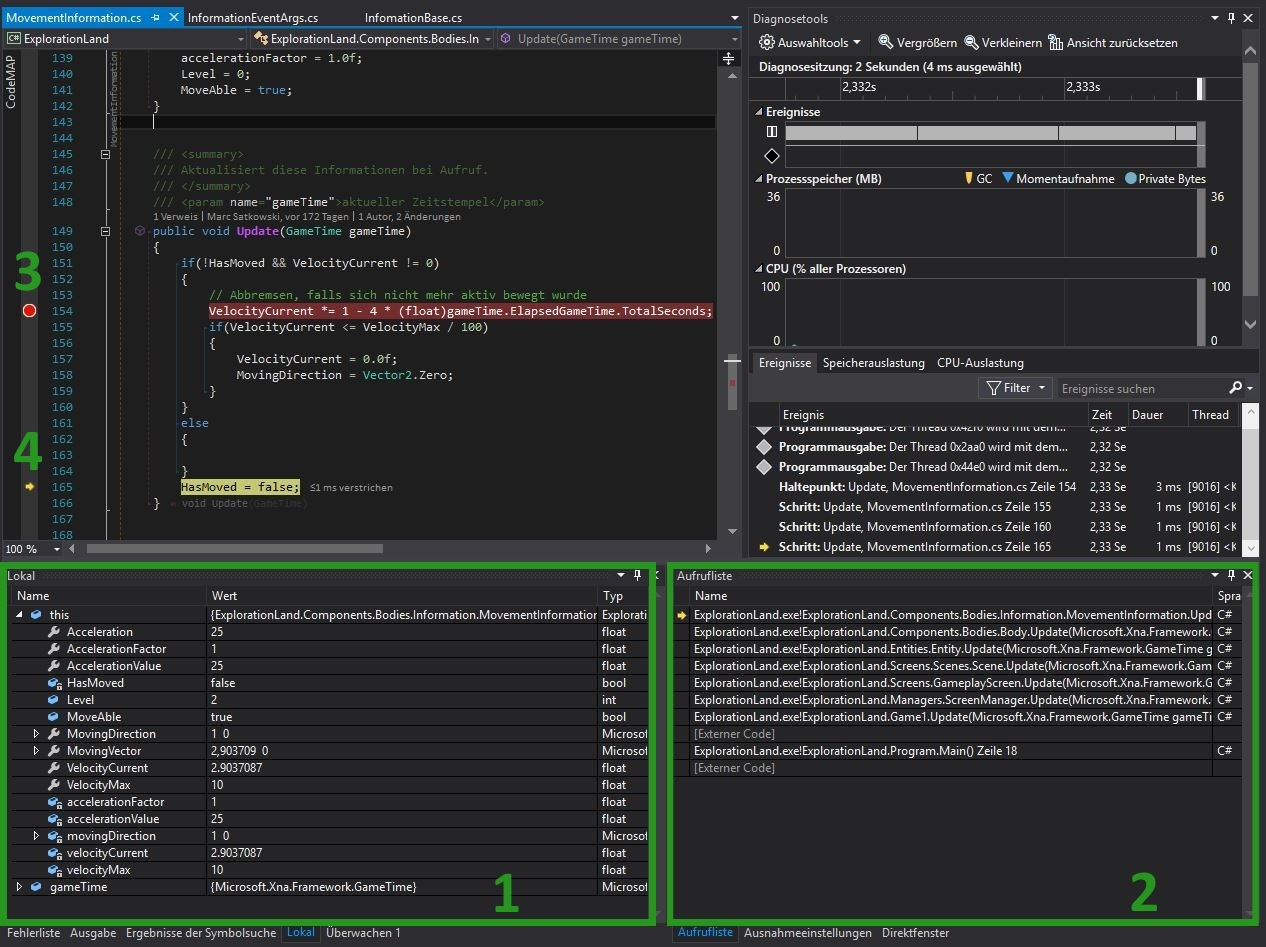
\includegraphics[scale=0.322]{resources/02_grundlagen_2/debugger.JPG}
	\end{figure}
\end{frame}

\begin{frame}{Beispiel: Visual Studio}
	\textbf{1 - Variablenanzeige:}
	\begin{itemize}
		\item Anzeige aller Variablen die gerade genutzt werden
		\item Dort kann man auch Daten verändern
	\end{itemize}
	\textbf{2 - Aufrufhierarchie:}
	\begin{itemize}
		\item Zeigt an von wo aus die jetzige Methode aufgerufen wurden ist
	\end{itemize}
	\textbf{3 - Haltepunkt:}
	\begin{itemize}
		\item Wie oben beschrieben
		\item Wird gesetzt durch einfaches klicken in die Leiste
	\end{itemize}
	\textbf{4 - Nächste auszuführende Zeile}
	\begin{itemize}
		\item Diese Zeile wird bei der nächsten schrittweisen Ausführen bearbeitet
	\end{itemize}
\end{frame}

\begin{frame}{Beispiel: Visual Studio}
	\begin{figure}
		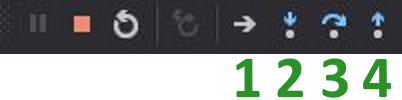
\includegraphics{resources/02_grundlagen_2/debugging.png}
	\end{figure}
	\begin{description}
		\item[1: ] Zeigt die nächste auszuführende Programmzeile an
		\item[2: ] Führt die nächste Zeile aus. Bei einer Methode wird in diese hineingegangen.
		\item[3: ] Führt die nächste Zeile aus.
		\item[4: ] Springt aus der jetzigen Methode heraus.
	\end{description}
\end{frame}

\end{document}
